% Преамбула
\documentclass[a4paper,14pt]{extarticle}
\usepackage[utf8]{inputenc}
\usepackage{graphicx}
\usepackage{indentfirst}
\usepackage[russian]{babel}
\usepackage{color}
\usepackage{float}
\usepackage[colorlinks,urlcolor=red,citecolor=blue,linkcolor=black,menucolor=black]{hyperref}
\usepackage{cite}
\usepackage{bm}
\usepackage{cmap}
\linespread{1.3}


%Параметры страницы
\textwidth 17cm
\textheight 23cm
\oddsidemargin 0cm
\topmargin -1cm
\def\Year{\expandafter\YEAR\the\year}
\def\YEAR#1#2#3#4{#3#4}
\renewcommand{\theequation}{\arabic{section}.\arabic{equation}}
\definecolor{grey}{gray}{0.3}

\begin{document}
\begin{titlepage}
\begin{center}
{\bf{Минобрнауки России}\\[14pt]
Федеральное государственное бюджетное образовательное учреждение
высшего образования \linebreak
«Омский государственный университет им.~Ф.М.~Достоевского»
}\\[2.2cm]
{\bf Ковалев Юрий Викторович}\\[2mm]
{\footnotesize \hspace*{11cm}{\color{grey}(подпись исследователя)}}\\[1cm]
{ \textbf{Отчет по производственной практике: курсовая работа}}\\[3cm]
\end{center}
\hspace*{6cm}{\bf Научный руководитель:}\\
\hspace*{7cm}{\bf д.ф.-м.н, профессор В.В.~Прудников}\\[18pt]
\hspace*{6cm}{\bf Заведующий кафедрой :}\\
\hspace*{7cm}{\bf д.ф.-м.н., профессор В.В.~Прудников}\\[2cm]

\begin{center}
{\bf Омск — 2019}
\end{center}
\end{titlepage}

\newpage
\tableofcontents

\newpage
\section*{Введение}
\addcontentsline{toc}{section}{Введение.} % Команда включающая название ненумеруемого раздела в ОГЛАВЛЕНИЕ
Поведение статистических систем вблизи температуры $T_C$ фазового перехода второго рода характеризуется чрезвычайно медленной динамикой с аномально большими временами релаксации, стремящимися к бесконечности как $t_{rel} \sim {|T - T_C|}^{-z\nu}$, где $z$ и $\nu$ - динамический критический индекс и индекс корреляционной длины соответственно.
В этих условиях система демонстрирует ряд особенностей своего неравновесного поведения, такие как явления старения и нарушения флуктуационно-диссипативной теоремы (\textbf{ФДТ}).
Эффекты старения наблюдаются только на временах $t << t_{rel}$ и проявляются в форме двухвременной зависимости корреляционной от времени наблюдения $t$ и времени ожидания $t_{\omega}$.
Целью данной работы является исследование критического поведения изотропной модели Гейзенберга. В исследование критического поведения входит:

\begin{itemize}
\item нахождение значения критической температуры $T_C$ для изотропной модели Гейзенберга с концентрацией спинов $P = 0.8$;
\item получение динамических зависимостей автокорреляционной функции $C(t,t_w)$ при компьютерном моделировании из низкотемпературного состояния с начальной намагниченностью $m_0 = 1$
\item Анализ влияния времени ожидания $t_w$ на временное поведение автокорреляционной функции;
\end{itemize}

%__________________________________________________________________________________________________

\newpage
\section{Получение значения $T_C$}

\subsection{Изотропная модель Гейзенберга}
В данной работе исследуются трехмерная изотропная модель Гейзенберга гамильтониан которой описывается, соответственно, следующим выражением
\begin{equation}
    H = -J \sum_{\langle i,j \rangle} p_ip_j\overrightarrow{S_i} \overrightarrow{S_j},
\end{equation}
где  $J$ – константа обменного взаимодействия, $J>0$ для ферромагнитной модели, $S_i^{x}$, $S_i^{y}$, $S_i^{z}$ - компоненты трехмерного вектора $\overrightarrow{S_i}$ , который находится в i-м узле решетки, $\langle i,j \rangle$ показывает, что суммирование идет по ближайшим соседям, $p$ - случайное число, принимающие значение $1$ или $0$, $p_i$ принимается равным $1$, если в $i$ узле находиться спин, и значение $0$, если спина в узле нет. 

\subsection{Методы исследования}
Для исследования трехмерной изотропной модели Гейзенберга требуется значение критической температуры $T_C$,  которое к началу исследования было неизвестно. Для нахождения значения критической температуры для данной модели используется метод кумулянтов Биндера.

\begin{equation}
U(L, T)=\frac{1}{2} \Biggl( 3-\frac{\langle M_4(T)\rangle}{{\langle M_2(T)\rangle}^2} \Biggr),
\end{equation}

 
 Компьютерное моделирования проводилось с помощью алгоритма Метрополиса. На решетку накладывались периодические граничные условия, которые устраняют влияние поверхностных эффектов и наилучшим образом соответствуют моделированию поведение объемных систем.

\subsection{Критическая температура}
Для получения $T_c$ проводилось компьютерное моделирование систем с линейными размерами $L = 24, 36, 48$. 
Для локализации $T_C$ был выбран интервал $T \in [1, 1.4]$, с шагом $\Delta T = 0.02$

\begin{figure}[H]
	\begin{center}
		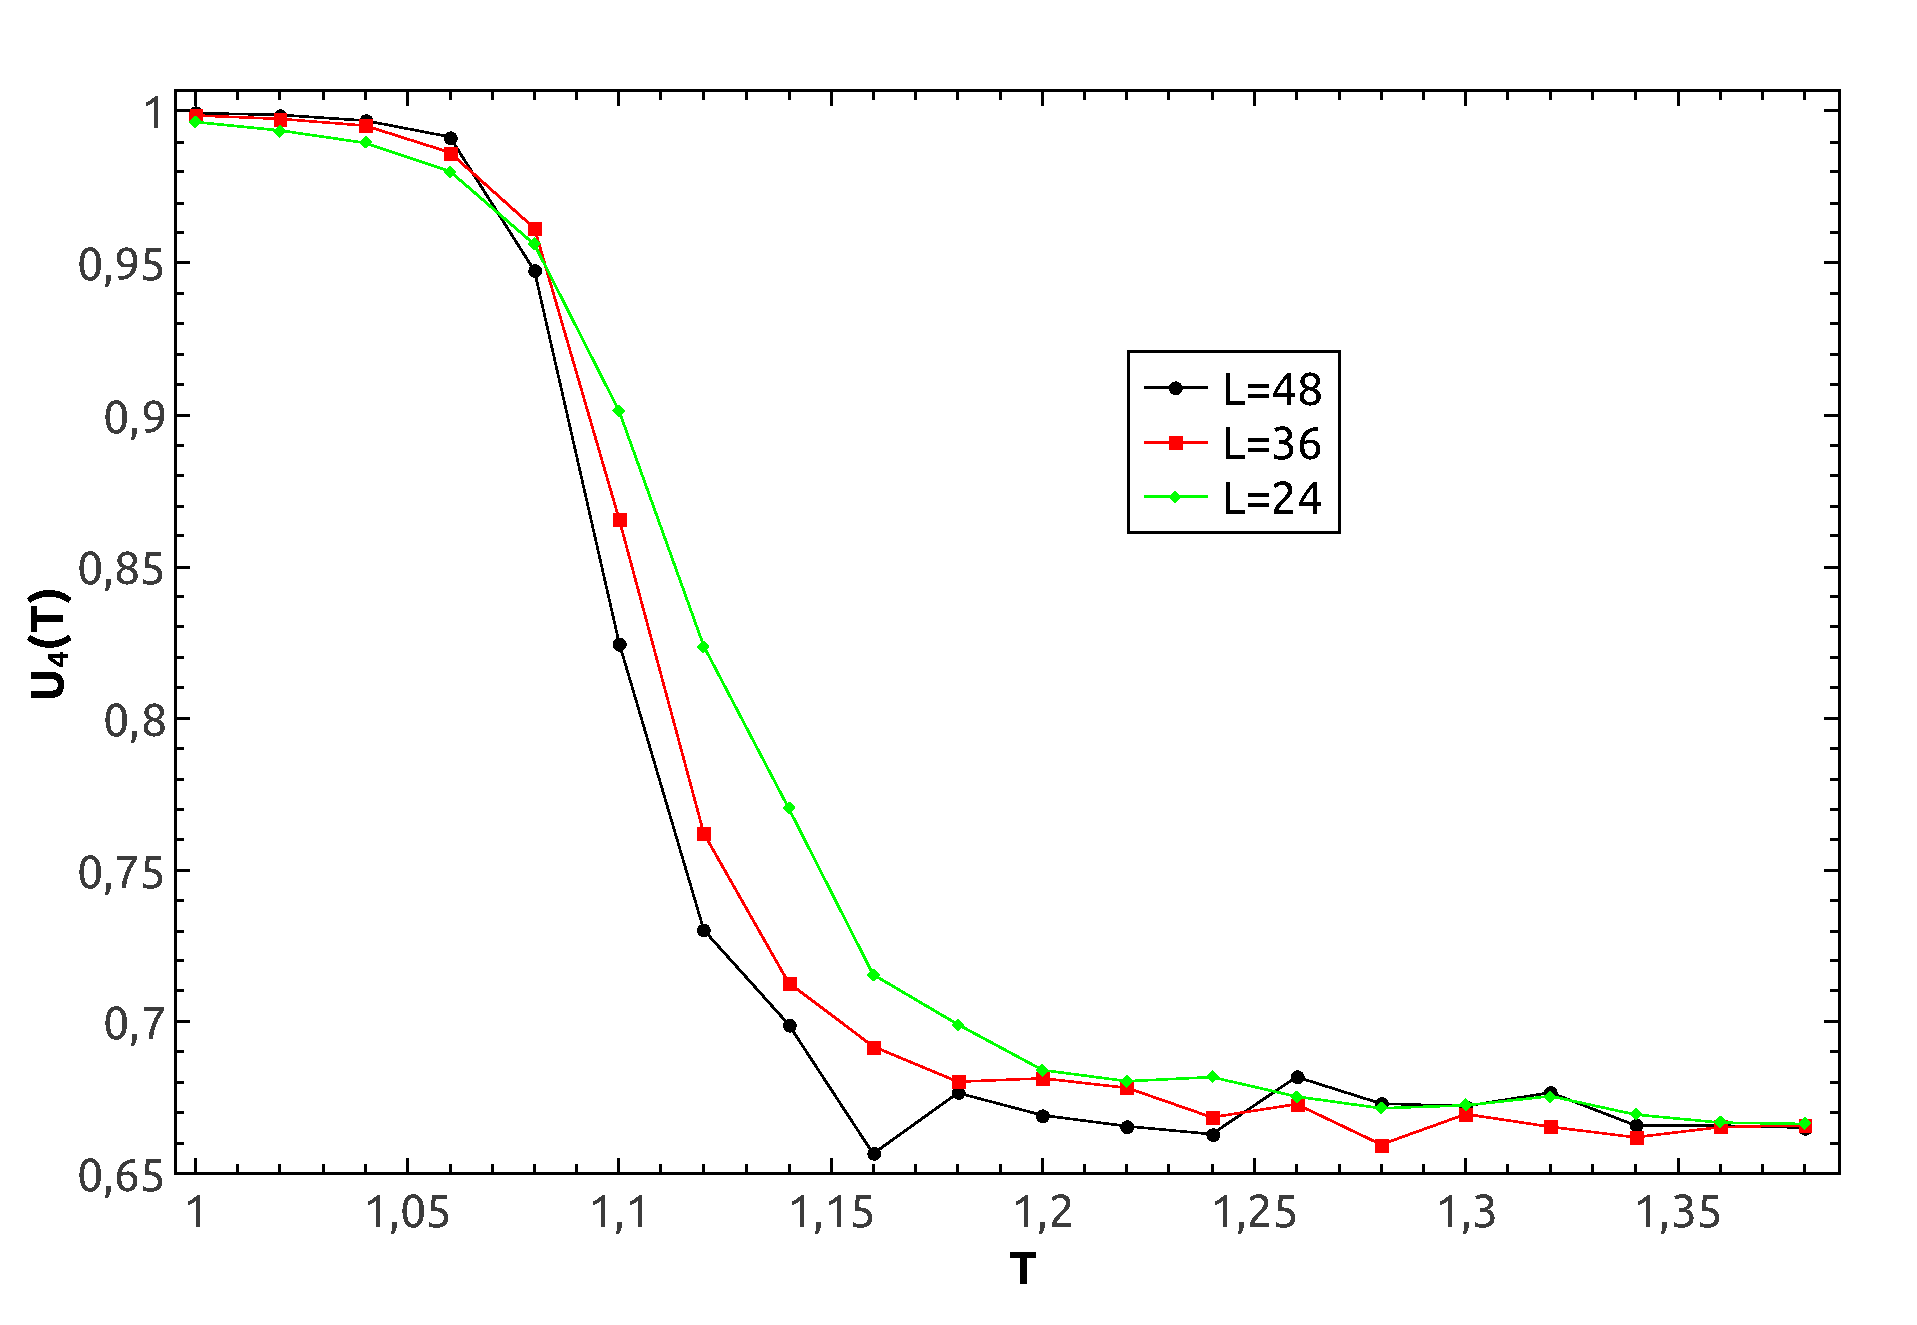
\includegraphics[width=0.99\textwidth]{kumfff.pdf}
		\caption{\label{testSolution} Температурная зависимость кумулянтов Биндера $U_4(L,T)$ для $L=24,36,48$.}
	\end{center}
\end{figure}

Для дальнейшего исследования была выбран интервал $T \in [1.07, 1.09]$ с шагом $\Delta T = 0.002$.
\begin{figure}[H]
	\begin{center}+++
		
		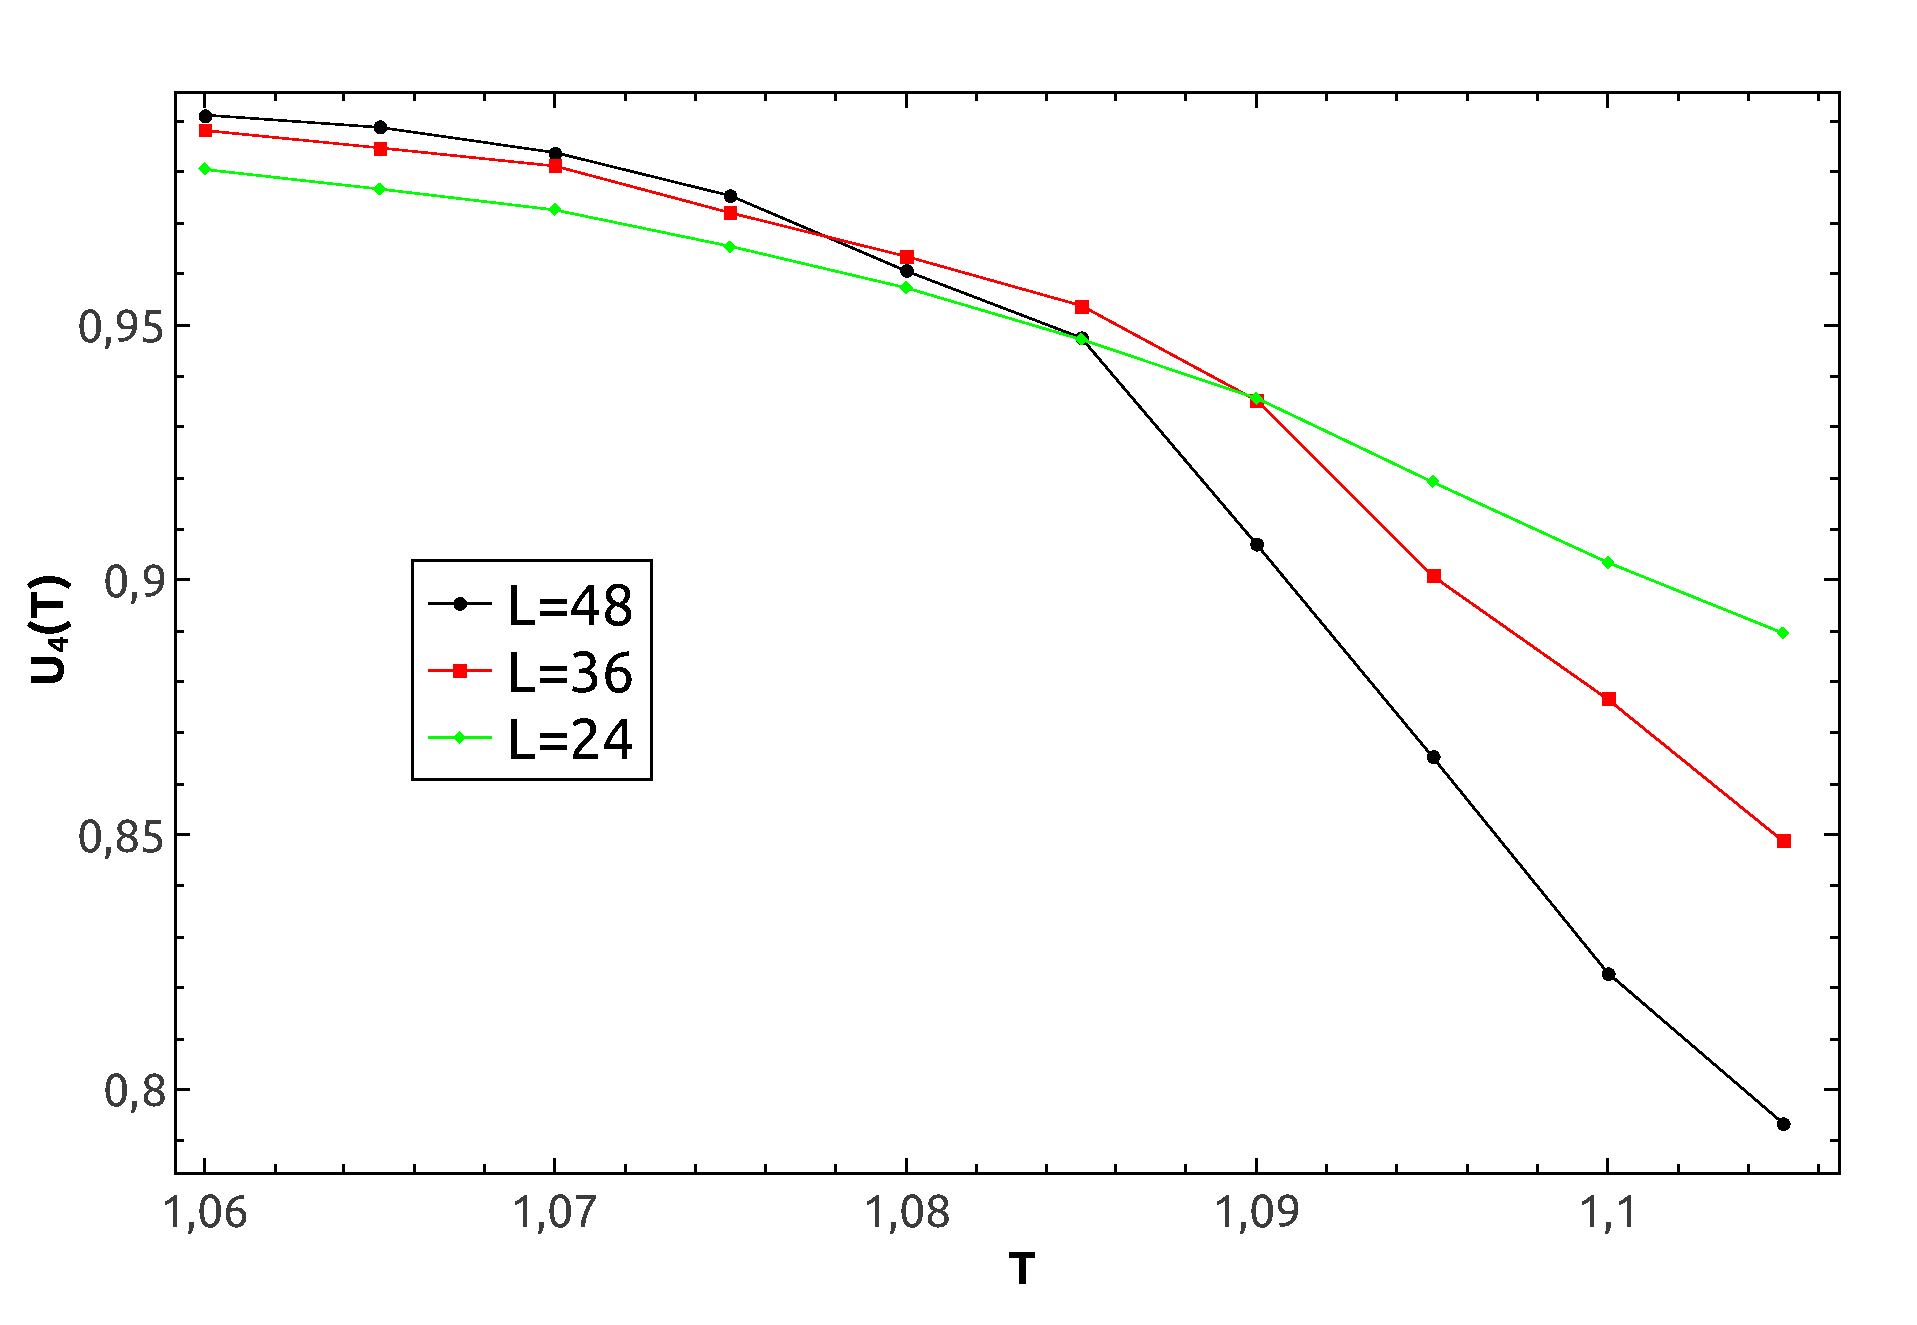
\includegraphics[width=0.49\textwidth]{kumsecond.pdf}
				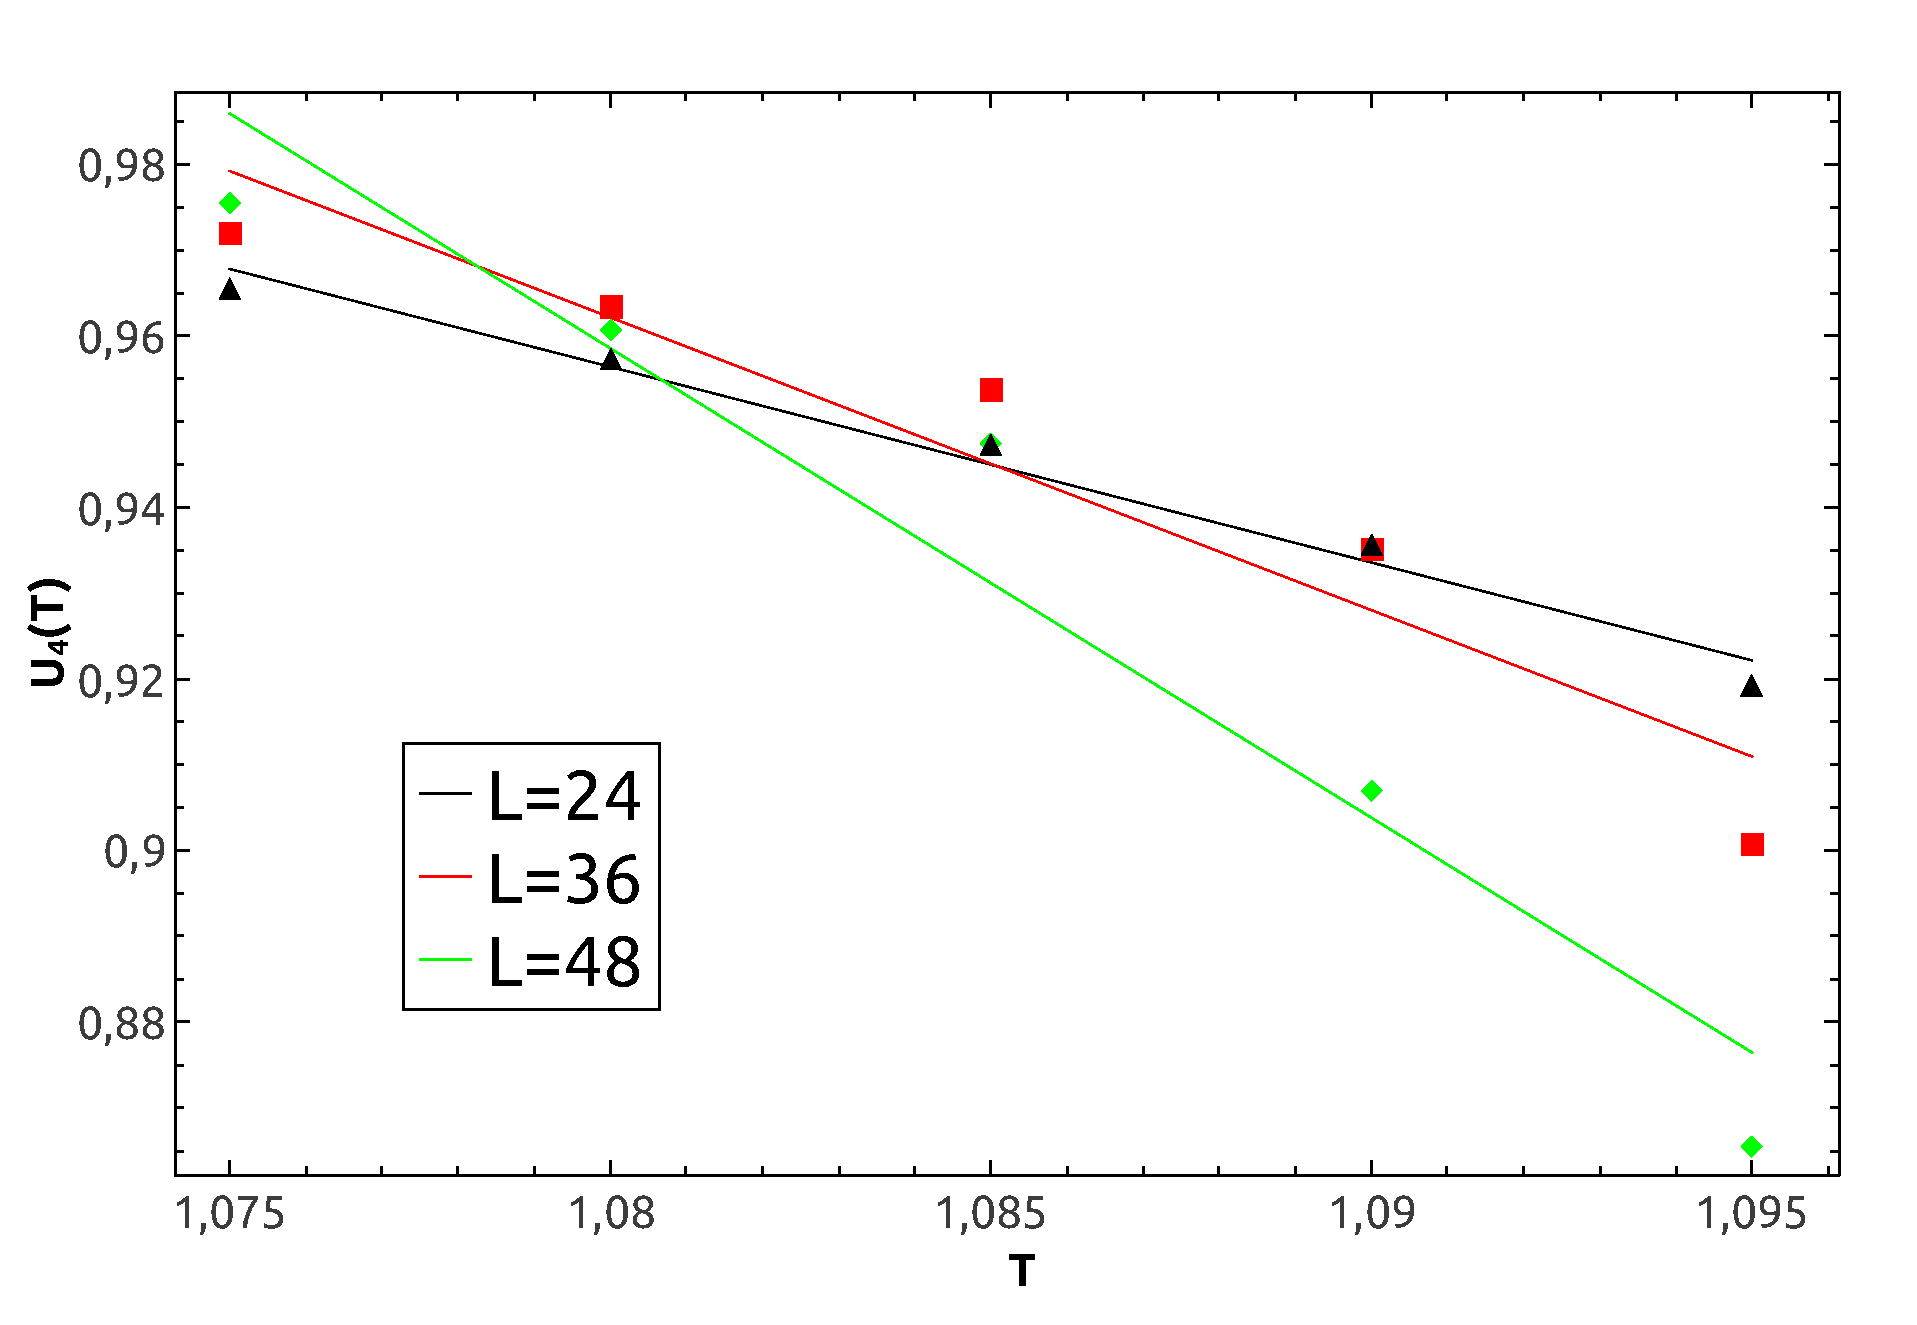
\includegraphics[width=0.49\textwidth]{kumfirst.pdf}
		\caption{\label{testSolution} Температурная зависимость кумулянтов Биндера $U_4(L,T)$ для $L=24,36,48$.}
	\end{center}
\end{figure}

Полученные кумулянты были аппроксимированы в интервале $T \in [1.075, 1.095]$ и было получено значение критической температуры $T_C = 1.0813(34)$

\section{Исследование автокорреляционной функции}
\subsection{Автокорреляционная функция}
В данном исследовании критических свойств изотропной модели Гейзенберга в качестве характеристики неравновесного процесса
используются такая величина, как двухвременная автокорреляционная функция
 
 \begin{equation}
   {C}(t,t_w) = \left\langle \frac{1}{N_s} \sum_{i=1}^{N_s} \overrightarrow{S_i}(t) \overrightarrow{S_i}(t_w) \right\rangle - \overrightarrow{M}(t) \overrightarrow{M}(t_w),
\end{equation}

где угловые скобки обозначают статистическое усреднение по реализациям начального состояния. Время ожидания $t_w$ характеризует отрезок
от момента приготовления образца до момента начала
измерения его характеристик.

\begin{figure}[h!]
	\begin{center}
		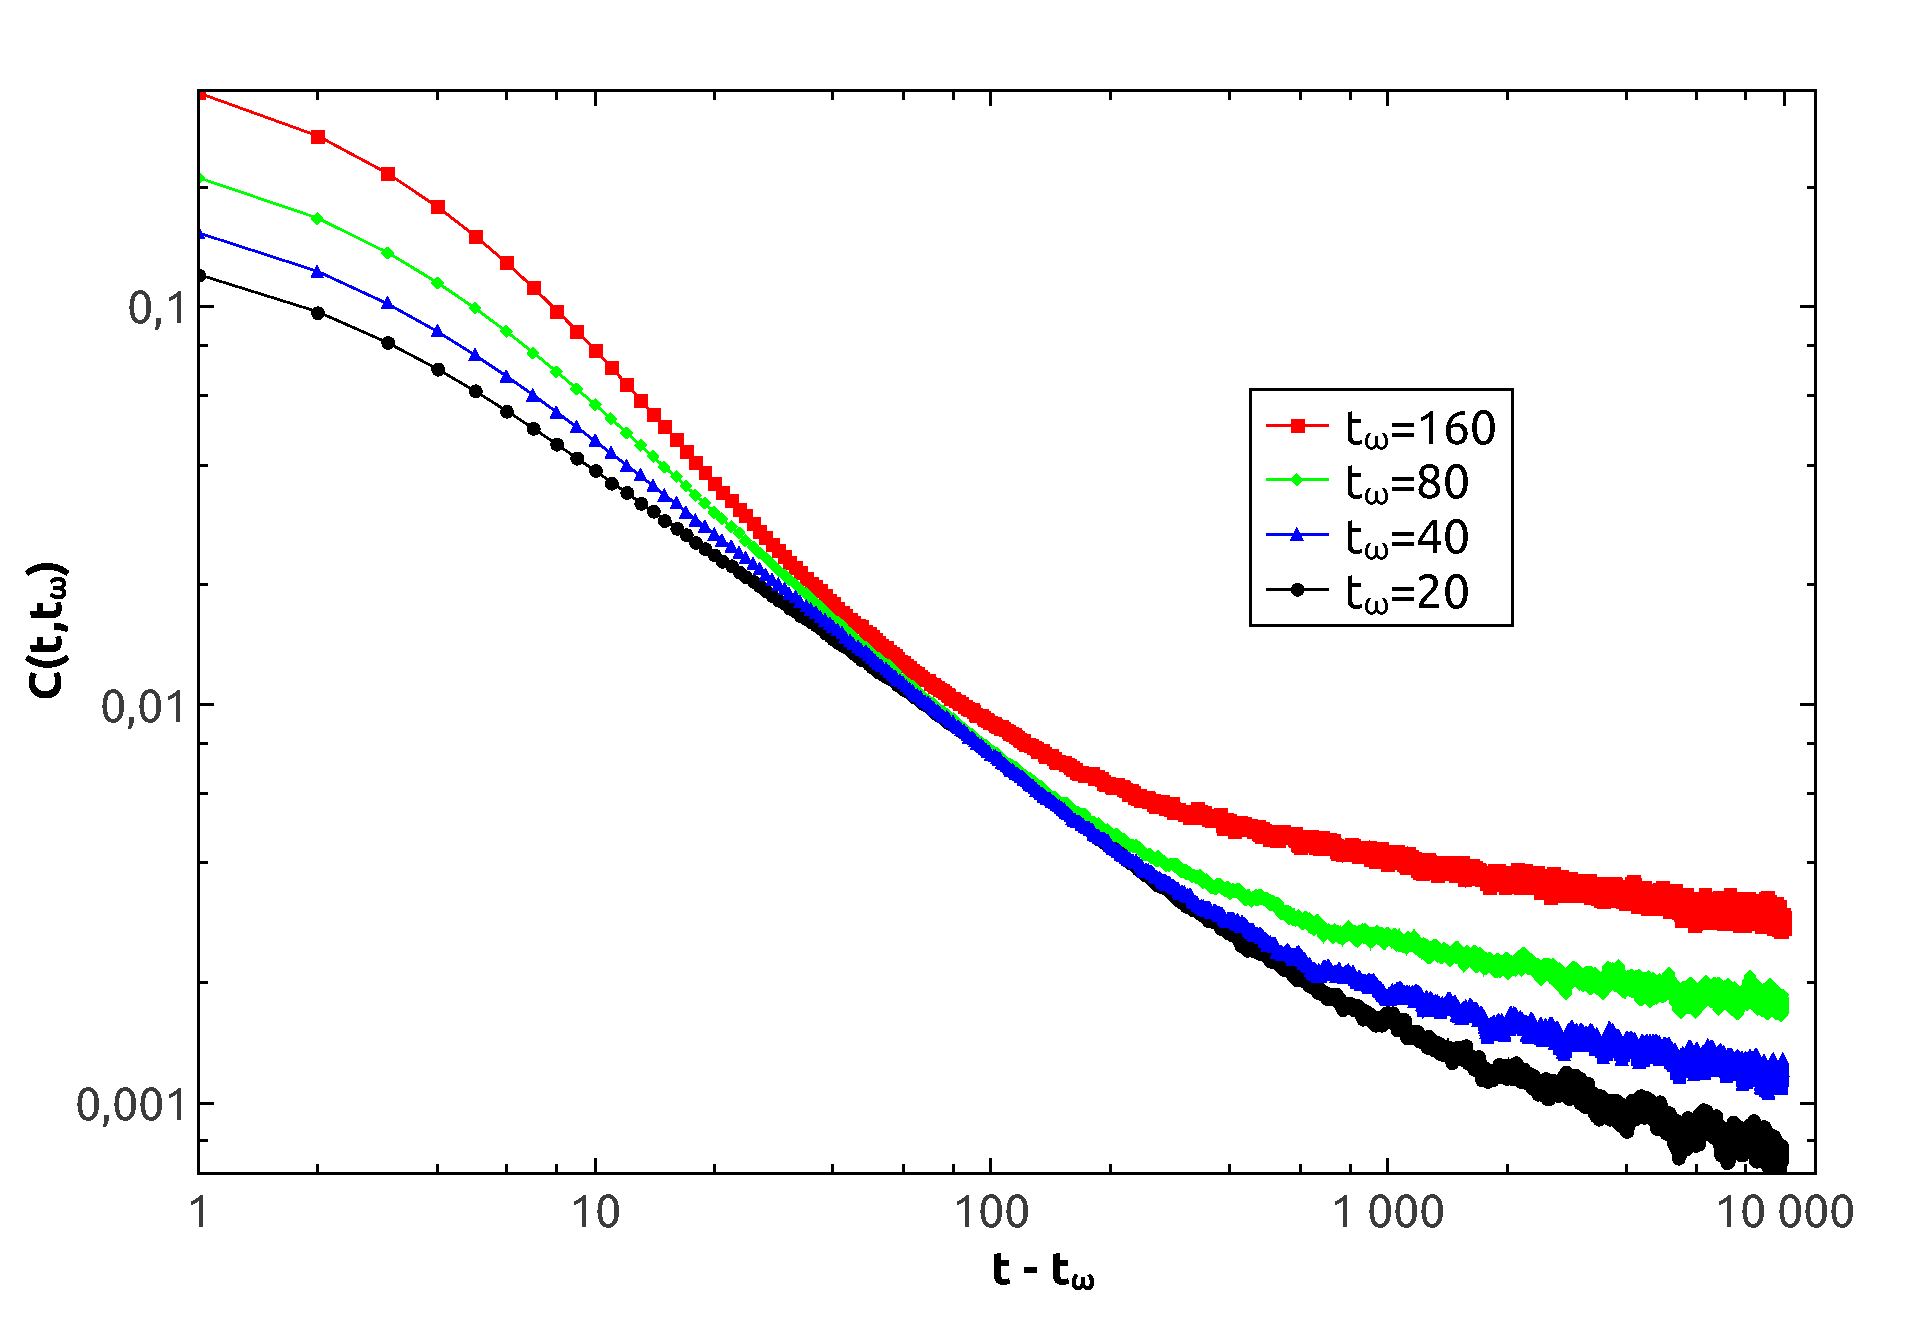
\includegraphics[width=0.99\textwidth]{C.pdf}
		\caption{\label{testSolution} Динамические зависимости автокорреляционной функции $C(t,t_w)$ при эволюции системы из низкотемпературного($m_0=1$) начального состояния при времени ожидания $t_w=20,40,80,160$ MCS.}
	\end{center}
\end{figure}

\newpage
\section*{Заключение}
\addcontentsline{toc}{section}{Заключение.}


Было проведено компьютерное моделирование для трехмерной изотропной модели Гейзенберга. проведено исследование:

\begin{itemize}
\item найдено значение критической температуры для анизотропной модели Гейзенберга с анизотропией типа легкая ось $T_c=1.0813(34)$;

\item Были получены динамические зависимости автокорреляционной функции $C(t,t_w)$ при компьютерном моделировании из низкотемпературного состояния с начальной намагниченностью $m_0 = 1$
\end{itemize}
\newpage
\begin{thebibliography}{99} \addcontentsline{toc}{section}{Литература.}

\bibitem{Vincent}
Прудников В.В., Прудников П.В., Лях А.С., Поспелов Е.А. Неравновесное критическое поведение трехмерной классической модели Гейзенберга // Вестн. Ом. ун-та. 2018. Т. 23, № 3. С. 64-72. DOI:10.25513/1812-3996.2018.23(3).64-72. 

\bibitem{Vincent}
Прудников В.В., Прудников П.В., Маляренко П.Н., Крижановский В.В. Влияние дефектов структуры на неравновесное критическое поведение трехмерной модели Изинга при эволюции из начального низкотемпературного состояния // Вестн. Ом. ун-та. 2015. № 4. С. 32-38. 


\end{thebibliography}
\end{document}

\documentclass[a4paper,14pt,russian]{extreport}
 
\usepackage{extsizes}
\usepackage{cmap} % для кодировки шрифтов в pdf
\usepackage[T2A]{fontenc}
\usepackage[utf8]{inputenc}
\usepackage[russian]{babel}
\usepackage{pscyr}
  
\usepackage{graphicx} % для вставки картинок
\usepackage{amssymb,amsfonts,amsmath,amsthm} % математические дополнения от АМС
\usepackage{indentfirst} % отделять первую строку раздела абзацным отступом тоже
\usepackage[usenames,dvipsnames]{color} % названия цветов
\usepackage{makecell}
\usepackage{multirow} % улучшенное форматирование таблиц
\usepackage{ulem} % подчеркивания
 
\linespread{1.3} % полуторный интервал
\renewcommand{\rmdefault}{ftm} % Times New Roman
\frenchspacing
